\subsection{Fast Eagle}
    \subsubsection{Definición}
      \paragraph{El módulo Fast Eagle formará parte de la arquitectura final de Ambienta2MX. El propósito principal de este módulo es brindar la información cartográfica de México por medio de un servicio expuesto, considerando latitud, longitud o nombre de la localidad deseada.}
      \paragraph{Fast Eagle se encargará de exposición de datos brindados por el (Instituto Nacional de Estadística y Geografía) INEGI considerando los datos públicos que tiene de la cartografía del territorio nacional.}
      \paragraph{Actualmente la información que proporciona el INEGI se encuentra en archivos de tipo CSV o bien, terceros se han encargado de estandarizar la información de forma relacional considerando MySQL como gestor principal de información.}
      \paragraph{Sin embargo, por la necesidad de búsquedas geográficas, se generó una migración de la información a un modelo de datos orientado a documentos, siguiendo la especificación GeoJSON en su versión del año 2008. Sólo basta con realizar un proceso de exportación al gestor de de documentos Mongo, y generar los índices geográficos. \cite{35}}
      \paragraph{La información que proporciona el INEGI carece de campos esenciales para la estandarización de la información cartográfica considerando el formato propuesto por el equipo de trabajo, para dar solución a ese contratiempo se hará uso de servicios externos que ya cuentan con información definida, es decir, que su información ha pasado bajo un cierto proceso de limpieza y regulación, por ejemplo, los servicios de Google Places API.}
      \paragraph{El objetivo principal de este módulo es brindar a los demás componentes del sistema información cartográfica de una localidad de país, considerando como valores de entrada, latitud y longitud o bien el nombre del lugar.}
      \paragraph{En caso de que no exista la información deseada por el usuario o algún otro módulo del sistema en la cartografía (base de datos llamada Places), Fast Eagle tratará de resolver la información en fuentes externas, persistiendo el modelo resuelto y regresando esa información al solicitante.}
    \subsubsection{Diagrama de clases}
    \begin{center}
      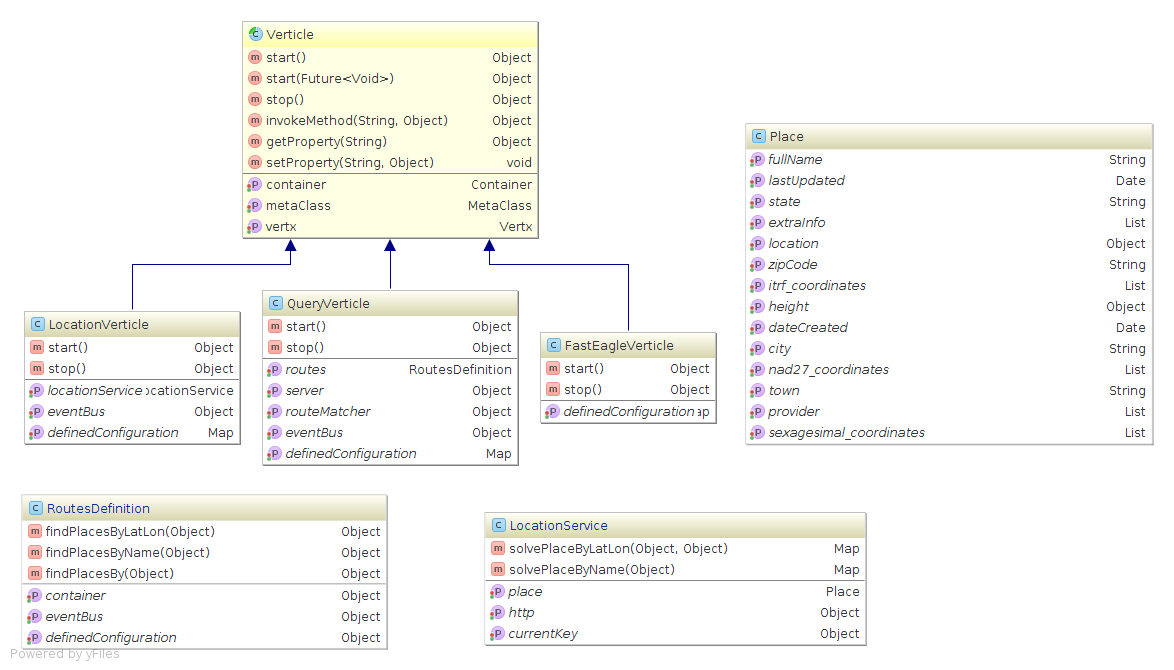
\includegraphics[width=16cm,height=10cm]{./images/FastEagleClassDiagram.png}
    \end{center}
    \newpage
    \subsubsection{Diagrama de sequencias}
    \begin{center}
      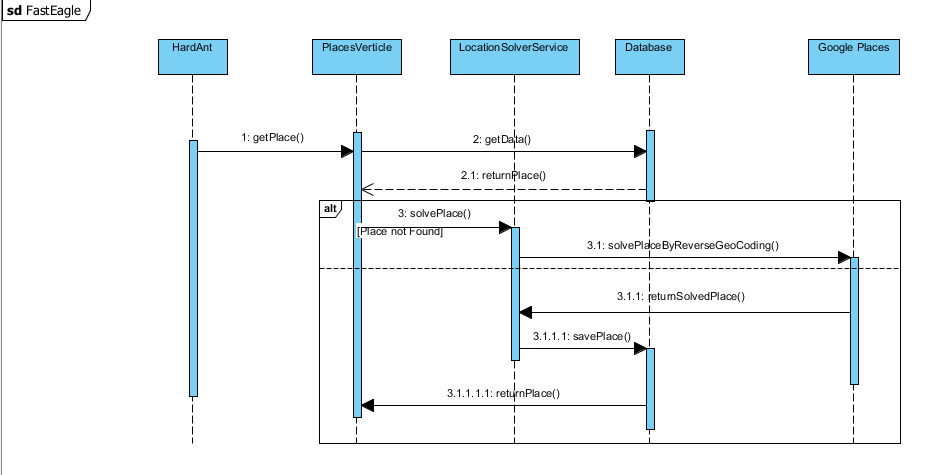
\includegraphics[width=16cm,height=10cm]{./images/FastEagleSequenceDiagram}
    \end{center}
    \subsubsection{Diagrama de bloques}
      \paragraph{Fast Eagle contará con varios procesos a ser desarrollados, la integración de cada proceso y su respectiva integración dará solución a un problema de estandarización, resolución y consulta de datos geográficos vía Latitud, Longitud y Ubicación.}
    \newpage
      \begin{landscape}
        \begin{figure}[b!]
        \centering
        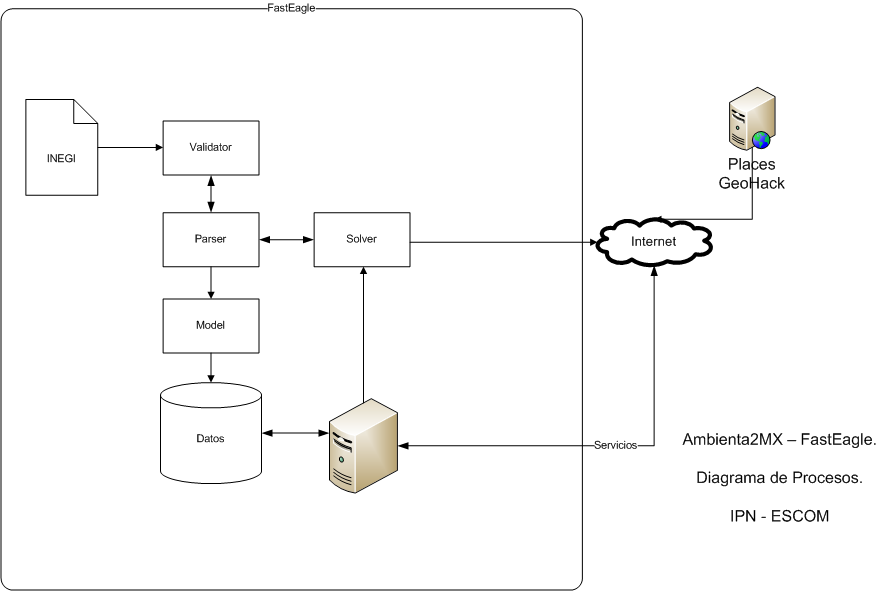
\includegraphics[width=22.5cm,height=12cm]{./images/DiagramaFastEagle.png}
        \caption{Diagrama por bloques de Fast Eagle}
      \end{figure}
      \end{landscape}
    \newpage
    \paragraph{En el diagrama se muestran tres módulos básicos, estos forman parte del núcleo de Fast Eagle, también podemos observar que se cuenta con la interacción de servicios de terceros como Google Places,  también se cuenta con la exposición de los servicios a través de un servidor web.}
    \paragraph{\textbf{\emph{Parser}} tomará los datos que el proceso de validación le arroje para transformar al estado propuesto por el equipo de trabajo (Véase modelo de datos). Considerando un proceso de resolución en caso de que la información proporcionada por el INEGI se encuentre incompleta no sea válida.}
    \paragraph{Para toda la información que carezca de datos correctos \textbf{\emph{Solver}} buscará una resolución en servicios de terceros, después de la resolución, los datos serán guardados en el gestor de bases de datos bajo el formato propuesto por el equipo de trabajo.}
    \paragraph{\textbf{\emph{Model}} es la capa de interacción con la base de datos, ésta se encarga de las operaciones mejor conocidas como CRUD (Create, Read, Update and Delete),  persistiendo la información en MongoDB, utilizando los canales de Vert.x para su convivencia con la antes mencionada.}
    \paragraph{Para poder exponer los datos, se hará uso de un servidor web minimalista orientado a micro servicios desarrollado en Vert.x, éste será un servicio público que formará parte de la infraestructura final de Ambienta2MX.}
    \paragraph{El servicio expuesto se encargará de las búsquedas a nivel base de datos y en caso de no encontrar la información buscará en terceros para poder agregarla a la base de datos y así ir mejorando el contenido de nuestro índice cartográfico.}
    \paragraph{Considerando las bondades que nos brinda el framework Vert.x, se generó un canal para la resolución de la información utilizando el servicio de Google Maps, éste canal interactua de forma directa con el servicio de places expuesto a todos los usuarios o módulos del sistema.}
    \paragraph{La comunicació principal será de tipo REST, para el proceso de obtención de información relacionada al territorio nacional.}